% --
% game kws integration

\section{Key Word Spotting System Integration}
\thesisStateReady
In order to use KWS in a video game, a dedicated system has to be integrated within the game framework.
The KWS system deployed in this thesis consists of two essential parts:
\begin{itemize}
	\item online system
	\item classification system
\end{itemize}
where the online system captures the audio stream input from a microphone in real-time and stores it in a FIFO (First In First Out) buffer for subsequent calculations of features and key word prediction in the classification system.
The classification system consists of a feature extractor and the neural network architecture for the KWS task.
The video game interprets the commands from the classification systems to real actions within the game.
More detailed descriptions of the individual sub systems are provided below.


% --
% online

\subsection{Online System}
The online system is mainly composed of a FIFO buffer for input data storage and an energy onset detection.
The length of the FIFO buffer must have at least the sample length of the speech command examples used to train the neural networks for classification.
The recorded files in the speech command dataset have a time duration of \SI{1}{\second}. 
Using this time duration however, would have made the classification of key words very slow and the gaming experience boring.
In this thesis, the length of a key word was restricted to \SI{500}{\milli\second} or 8000 samples.
Further some buffer samples were added for an improved detection of the highest energy region within the speech signal.
Note that the input stream reads out the microphone data in chunk, where the length of each chunk was chosen to 160 samples, corresponding to exactly one frame with hop size of \SI{10}{\milli\second}.
Ideally these buffer frames should not be necessary, but due to shift invariance problems in some network architectures (especially for the \texttt{fstride} model), it can be advantageous and improve the key word predictions when buffer frames are added.

The buffer frames are located prior and posterior to the dedicated key word frames and were selected to both 5 frames for the prior and posterior buffer.
The frames for the prior buffer are collected consecutively from the audio stream and are updated to the size of the prior buffer. 
Each input chunk or frame is used for the detection of an online onset as described in \rsec{signal_onset_online}.
If an onset is detected from one of these frames, subsequently the FIFO will be filled up to its full size including the posterior buffer frames.
Afterwards the whole FIFO is read out and the obtained frames are passed to the feature extraction module already located in the classification system.
The scheme of the online system with integrated FIFO buffer is illustrated in \rfig{game_system_online}.
\begin{figure}[!ht]
  \centering
  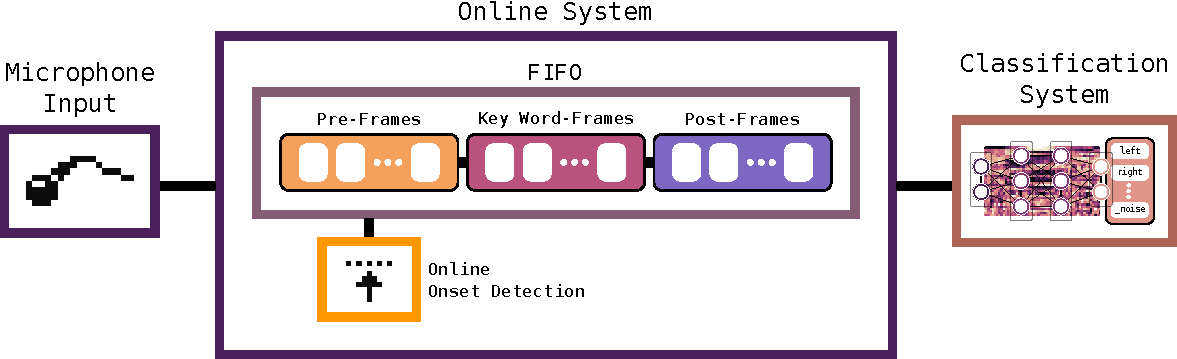
\includegraphics[width=0.60\textwidth]{./6_game/figs/game_system_online.pdf}
  \caption{Scheme of the online system with FIFO structure.}
  \label{fig:game_system_online}
\end{figure}
\FloatBarrier
\noindent


% --
% classification

\subsection{Classification System}
The classification system consists of a feature extractor and a classifier, which is composed of a neural network architecture for the classification of the key words it was trained for.
The feature extractor computes the MFCCs according to its provided feature extraction parameters and determines the highest energy onset as described in \rsec{signal_onset_kw}.
The feature extraction parameters provide information about the exact constellation of features used during training, for instance 12 MFCC coefficients with frame-based normalization and no feature enhancements.
This ensures, that the same feature extraction is applied to new data frames from the online system.

The classifier requires the unique name of the trained neural network model (for example \texttt{conv-jim}), the parameters of this model and the class dictionary.
The trained weights of the  models are stored in the \texttt{.pth} format of the \texttt{Pytorch} framework and can simply be loaded to a corresponding model architecture.
The class dictionary describes which output node of the neural network corresponds to which speech command and is especially important for the video game to trigger correct actions.
After the parameters are loaded, the classifier simply performs an inference to the most probable key word in its class dictionary.

A game action is elicited, once a key word is present from the classification system.
This for example, can be implemented by using an input handler, similar to a keyboard input handler or event system, that is listening for new speech commands and does trigger an action when one is available.
A simple scheme of the classification system is shown in \rfig{game_system_classification}.
\begin{figure}[!ht]
  \centering
  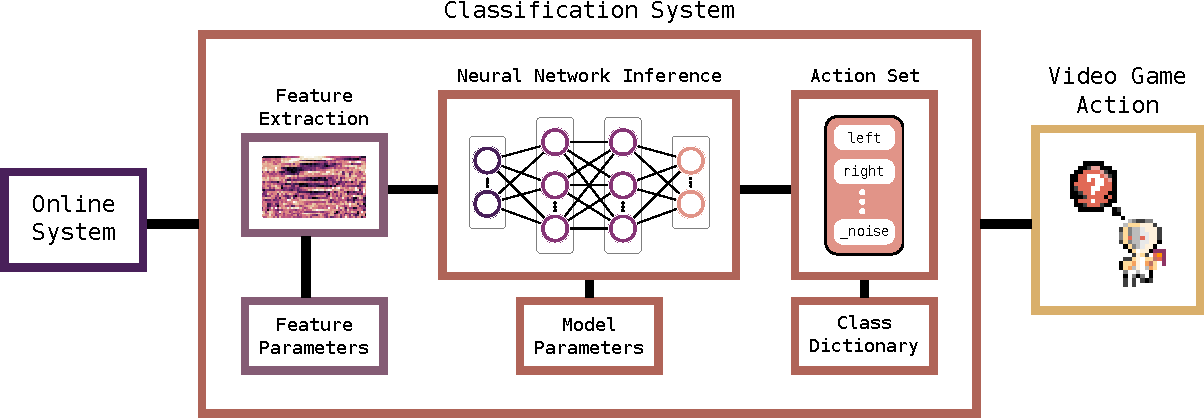
\includegraphics[width=0.65\textwidth]{./6_game/figs/game_system_classification.pdf}
  \caption{Scheme of the classification system.}
  \label{fig:game_system_classification}
\end{figure}
\FloatBarrier
\noindent

